\chapter{Introduction}

\section{Definitions}

$P(t,T)$ denotes the price at time $t$ of a zero-coupon bond maturing at time $T$. 
For a fixed $t$, $P(t,T)$ is referred to as the term structure of discount bonds 
at time $t$, or the discount curve at time $t$.
The discount curve is related to the continuously compounded yield curve $y$ by
\begin{equation}
P(t,T) = \e^{-y(t,t,T) (T - t)}.
\end{equation}

Likewise the discount curve is related to the instantaneous forward rate $f$
\begin{equation}
P(t,T) = \exp \left( -\int_t^T f(t,u) du \right),
\end{equation}
hence
\begin{eqnarray}
f(t,T) &=& - \frac{\partial \ln P(t,T)}{\partial T} \\
&=& y(t,t,T) + \frac{\partial y(t,t,T)}{\partial T} (T - t).
\end{eqnarray}

\begin{figure}
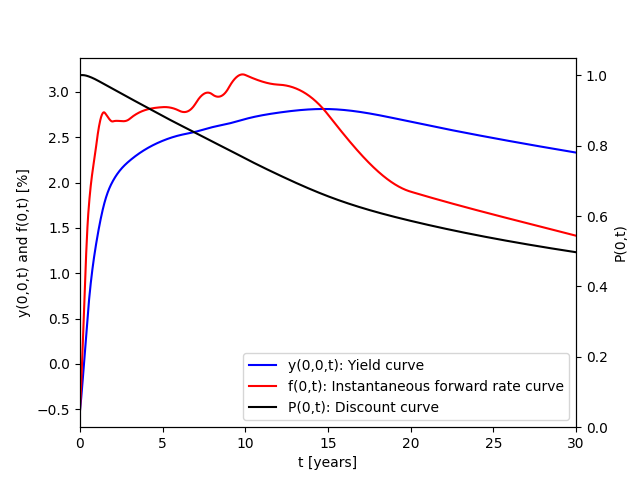
\includegraphics[scale=0.7]{figures/swap_curve.png}
\caption{Initial yield curve, instantaneous forward rate curve, and 
discount curve.}
\end{figure}
